\documentclass[a4paper]{article}
\usepackage[utf8]{inputenc}
\usepackage{amsmath}
\usepackage{amssymb}
\usepackage{mathtools}
\usepackage{amsfonts}
\usepackage{lastpage}
\usepackage{tikz}
\usepackage{float}
\usepackage{textcomp}
\usetikzlibrary{patterns}
\usepackage{pdfpages}
\usepackage{gauss}
\usepackage{fancyvrb}
\usepackage[table]{colortbl}
\usepackage{fancyhdr}
\usepackage{graphicx}
\usepackage[margin=2.5 cm]{geometry}

\definecolor{listinggray}{gray}{0.9}
\usepackage{listings}
\lstset{
	language=,
	literate=
		{æ}{{\ae}}1
		{ø}{{\o}}1
		{å}{{\aa}}1
		{Æ}{{\AE}}1
		{Ø}{{\O}}1
		{Å}{{\AA}}1,
	backgroundcolor=\color{listinggray},
	tabsize=3,
	rulecolor=,
	basicstyle=\scriptsize,
	upquote=true,
	aboveskip={0.2\baselineskip},
	columns=fixed,
	showstringspaces=false,
	extendedchars=true,
	breaklines=true,
	prebreak =\raisebox{0ex}[0ex][0ex]{\ensuremath{\hookleftarrow}},
	frame=single,
	showtabs=false,
	showspaces=false,
	showlines=true,
	showstringspaces=false,
	identifierstyle=\ttfamily,
	keywordstyle=\color[rgb]{0,0,1},
	commentstyle=\color[rgb]{0.133,0.545,0.133},
	stringstyle=\color[rgb]{0.627,0.126,0.941},
  moredelim=**[is][\color{blue}]{@}{@},
}

\lstdefinestyle{base}{
  emptylines=1,
  breaklines=true,
  basicstyle=\ttfamily\color{black},
}

\pagestyle{fancy}
\def\checkmark{\tikz\fill[scale=0.4](0,.35) -- (.25,0) -- (1,.7) -- (.25,.15) -- cycle;}
\newcommand*\circled[1]{\tikz[baseline=(char.base)]{
            \node[shape=circle,draw,inner sep=2pt] (char) {#1};}}
\newcommand*\squared[1]{%
  \tikz[baseline=(R.base)]\node[draw,rectangle,inner sep=0.5pt](R) {#1};\!}
\newcommand{\comment}[1]{%
  \text{\phantom{(#1)}} \tag{#1}}
\def\el{[\![}
\def\er{]\!]}
\def\dpip{|\!|}
\def\MeanN{\frac{1}{N}\sum^N_{n=1}}
\cfoot{Page \thepage\ of \pageref{LastPage}}
\DeclareGraphicsExtensions{.pdf,.png,.jpg}
\author{Nikolaj Dybdahl Rathcke (rfq695)}
\title{Machine Learning \\ Assignment 2.2}
\lhead{Machine Learning}
\rhead{Assignment 2.2}

\begin{document}
\maketitle

\section{Principal Component Analysis}

\subsection{Summarization by the mean}
We want to find the $b$ that minimizes the entire sum. This is done by taking the derivative with respect to $b$, so we want to solve the following:
\begin{align*}
\nabla_b \left(\frac{1}{N}\sum_{i=1}^N \dpip x_i-b \dpip^2\right)=0
\end{align*}
We can calculate the gradient on the left side after rewriting $\dpip x_i-b\dpip^2$ to $(x_i-b)^2$, to get:
\begin{align*}
\nabla_b \left(\frac{1}{N}\sum_{i=1}^N (x_i-b)^2\right)&=\frac{1}{N}\sum_{i=1}^N 2(b-x_i) \\
&=\frac{2}{N}\sum_{i=1}^N (b-x_i) \\
&=\frac{2}{N}\sum_{i=1}^N b-\frac{2}{N}\sum_{i=1}^N x_i \\
&=\frac{2Nb}{N}-\frac{2}{N}\sum_{i=1}^N x_i \\
&=2b-\frac{2}{N}\sum_{i=1}^N x_i \\
\end{align*}
We can now solve it for zero and move the sum (and the fraction) to the other side:
\begin{align*}
2b-\frac{2}{N}\sum_{i=1}^N x_i &=0\ \Leftrightarrow\ 2b=\frac{2}{N}\sum_{i=1}^N x_i \ \Leftrightarrow\ b=\frac{1}{N}\sum_{i=1}^N x_i
\end{align*}
Which is wanted to show. We know it is a minimum as it is a convex second degree polynomial, so it only has one extremum which is of minimum value.

\subsection{PCA for high dimensional data and small samples}
N/A

\subsection{Cybercrime Detection}
The code that performs the PCA is implemented in \texttt{src\_pca.py}. Running that file will produce the eigenspectrum and the scatterplot. The eigenspectrum when plotted with a logarithmic y-scale will look like this:
\begin{center}
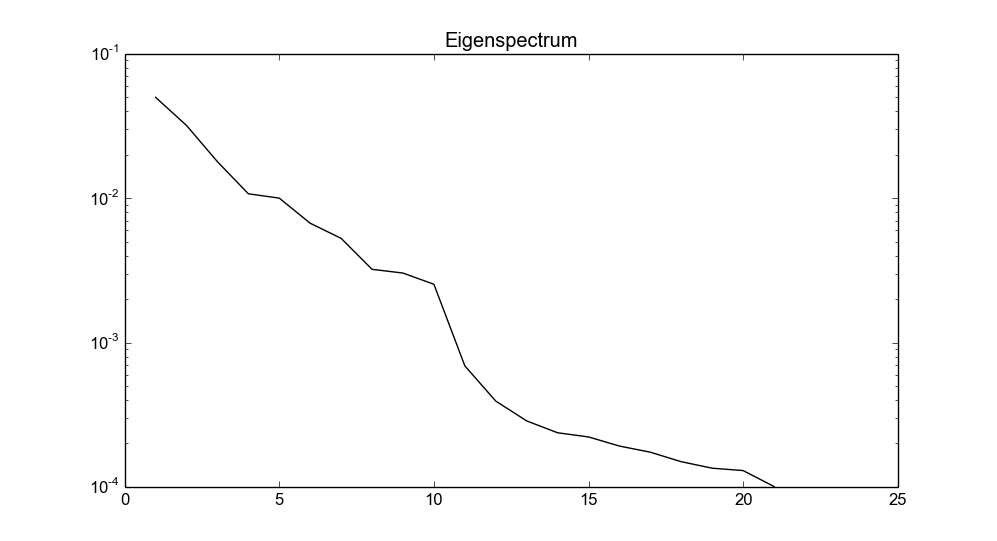
\includegraphics[scale=0.5]{fig2}
\end{center}
We can see that using more than around $10$ or $11$ principal components is a bit of a waste as there is a significant drop. \\
The scatterplot we get will look like this:
\begin{center}
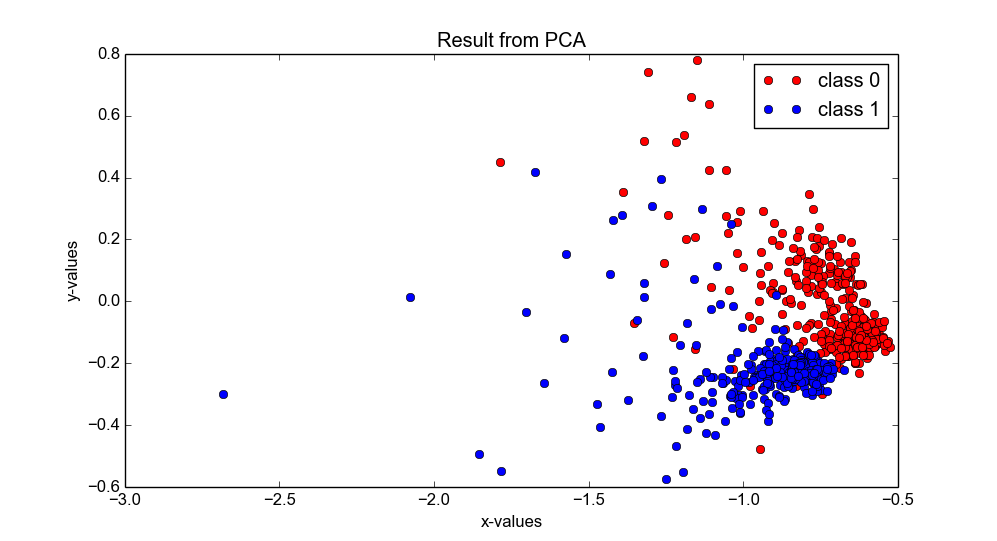
\includegraphics[scale=0.5]{fig1}
\end{center}
where the red dots is the ones with class $0$ and the blue dots are those with class $1$. As we can see, when the data is projected on the first two principal components they are already quite nicely divided.

\section{Occam’s Razor}

\subsection{}
We use corollary 2.4 from the lecture notes on Occam's Razor bound, with $M=2^{27^d}$, to bound $L(h)-\hat{L}(h,S)$:
\begin{align*}
\mathbb{P}\left\{ \exists h \in \mathcal{H}:L(h)-\hat{L}(h,S)\geq \sqrt{\frac{\ln(2^{27^d}/\delta)}{2n}}\right\}\leq \delta
\end{align*}
Where we have moved $\hat{L}(h,S)$ to the left side of inequality and $M=2^{27^d}$ because we have $27^d$ words of length $d$, so there must be $2^{27^d}$ subsets of this, which is the cardinality of the hypotheses space.

\subsection{}
We use theorem 2.5 from the lecture notes, where we do not use it for binary decision trees, but for trees that branch in $27$, so
\begin{align*}
\mathbb{P}\left\{ \exists h \in \mathcal{H}:L(h)-\hat{L}(h,S)\geq \sqrt{\frac{\ln(2^{27^{d(h)}}27^{d(h)}/\delta)}{2n}}\right\}\leq \delta
\end{align*}
where we again moved $\hat{L}(h,S)$ to the left side of the equation and $d(h)$ is the depth function, i.e. just $d$.

\end{document}
